\documentclass[nofootinbib,amssymb,amsmath]{revtex4}
\usepackage{mathtools}
\usepackage{amsthm}
\usepackage{amsmath}
\usepackage{algorithm}
\usepackage{algpseudocode}
\usepackage{lmodern}
\usepackage{graphicx}
\usepackage{color}
\usepackage{bm}

\usepackage{xcolor}
\usepackage{listings}
\lstset{basicstyle=\ttfamily,
  showstringspaces=false,
  commentstyle=\color{gray},
  keywordstyle=\color{blue},
  captionpos=b
}

%Put an averaged random variable between brackets
\newcommand{\ave}[1]{\left\langle #1 \right\rangle}

\newcommand{\vzero}{{\bf 0}}
\newcommand{\vI}{{\bf I}}
\newcommand{\vb}{{\bf b}}
\newcommand{\vd}{{\bf d}}
\newcommand{\vf}{{\bf f}}
\newcommand{\vc}{{\bf c}}
\newcommand{\vv}{{\bf v}}
\newcommand{\vz}{{\bf z}}
\newcommand{\vn}{{\bf n}}
\newcommand{\vm}{{\bf m}}
\newcommand{\vG}{{\bf G}}
\newcommand{\vQ}{{\bf Q}}
\newcommand{\vM}{{\bf M}}
\newcommand{\vW}{{\bf W}}
\newcommand{\vX}{{\bf X}}
\newcommand{\vPsi}{{\bf \Psi}}
\newcommand{\vSigma}{{\bf \Sigma}}
\newcommand{\vlambda}{{\bf \lambda}}
\newcommand{\vpi}{{\bf \pi}}
\newcommand{\valpha}{{\bm{\alpha}}}
\newcommand{\vbeta}{{\bm{\beta}}}
\newcommand{\vomega}{{\bm{\omega}}}
\newcommand{\vLambda}{{\bf \Lambda}}
\newcommand{\vA}{{\bf A}}

\newcommand{\code}[1]{\texttt{#1}}
\newcommand*{\Comb}[2]{{}^{#1}C_{#2}}

\newtheorem{lemma}{Lemma}
\newtheorem{corollary}{Corollary}

\def\SL#1{{\color [rgb]{0,0,0.8} [SL: #1]}}
\def\DB#1{{\color [rgb]{0,0.8,0} [DB: #1]}}

\newcommand{\HOM}{$\mathsf{Hom}$}
\newcommand{\HET}{$\mathsf{Het}$}
\newcommand{\REF}{$\mathsf{Ref}$}
\newcommand{\epss}{\varepsilon}

\begin{document}

\title{Notes on Mutect2}
\author{David Benjamin}
\email{davidben@broadinstitute.org}
\affiliation{Broad Institute, 415 Main Street, Cambridge, MA 02142}
\author{Takuto Sato}
%\email{tsato@broadinstitute.org}
\affiliation{Broad Institute, 415 Main Street, Cambridge, MA 02142}
\author{Lee Lichtenstein}
%\email{lichtens@broadinstitute.org}
\affiliation{Broad Institute, 415 Main Street, Cambridge, MA 02142}
\author{Megan Shand}
%\email{mshand@broadinstitute.org}
\affiliation{Broad Institute, 415 Main Street, Cambridge, MA 02142}

\date{\today}

\maketitle

%%%%%%
%%%%%%
%MUTECT2
%%%%%%
%%%%%%
\section{Mutect2}
Here we describe the command-line program \code{Mutect2} itself, which takes us from aligned reads to unfiltered, annotated variant calls.  Code block \ref{cmd-mutect2} shows how to invoke \code{Mutect2} using the gatk launch script.

\begin{lstlisting}[language=bash,caption={Mutect2 command}, label={cmd-mutect2}]
gatk Mutect2 -R reference.fasta \
   -L intervals.interval_list \
   -I tumor1.bam \
   # Mutect2 may input more tumor samples from the same individual 
   [-I tumor2.bam -I tumor3.bam . . .]  \
   # Mutect2 may input matched normals from the same individual
   [-I normal1.bam -I normal2.bam . . .]  \
   # For most purposes Mutect2 should be supplied with gnomAD
   [-germline-resource af-only-gnomad.vcf] \
    # Mutect2 may input a panel of normals to help identify technical artifacts
   [-pon panel_of_normals.vcf ]  \
   # Mutect2 may output orientation bias data
   # for LearnReadOrientationModel
   [--f1r2-tar-gz f1r2.tar.gz] \
   -O unfiltered.vcf
\end{lstlisting}

%%%%%
%MODES
%%%%%
\subsection{Additional modes}
The command above encompasses tumor-only, tumor-normal, and multiple-tumor somatic variant calling.  

\subsubsection{Mitochondria mode}
For mitochondrial calling one should add the \code{--mitochondria-mode} flag to the \code{Mutect2} command line.  This switches several defaults from values appropriate to somatic variant calling to values that reflect the greater density of mitochondrial mutations.  It also activates annotations relevant to alignment artifacts involving nuclear paralogs to mitochondrial DNA.

\subsubsection{Force calling}
One can force \code{Mutect2} to assemble and genotype all the variants in force-calls.vcf by adding \code{--genotyping-mode GENOTYPE\_GIVEN\_ALLELES -alleles force-calls.vcf} to the command line.  This injects all alleles in force-calls.vcf into the assembly graph, deactivates pruning of subgraphs contained them, and forces \code{Mutect2} to emit them in the output vcf regardless of their evidence.  In order to include even filtered alleles in force-calls.vcf, use the \code{--genotype-filtered-alleles} flag.  Force-called alleles are emitted \textit{in addition} to any alleles that \code{Mutect2} would otherwise discover.  This so-called GGA mode is useful for studying known driver mutations, for monitoring tumors after chemotherapy, and for validating calls from \code{Mutect2} or other tools against some orthogonal sequencing data.

%%%%%%%%%%%%%%%%%%%%
%ACTIVE REGION DETERMINATION
%%%%%%%%%%%%%%%%%%%%
\subsection{Finding Active Regions}
\code{Mutect2} triages sites based on their pileup at a single base locus.  If there is sufficient evidence of variation \code{Mutect2} proceeds with local reassembly and realignment.  As in the downstream parts of \code{Mutect2} we seek a likelihood ratio between the existence and non-existence of an alt allele.  Instead of obtaining read likelihoods via Pair-HMM, we assign each base a likelihood.  For substitutions we can simply use the base quality.  For indels we assign a heuristic effective quality that increases with length.

We use a version of the somatic likelihoods model, described below, with the following modifications:
\begin{itemize}
\item We treat every ref base as completely certain.  That is, $\ell_{r,{\rm ref}} = 1$ for ref bases.
\item We combine all alt alleles and reads supporting them into a single effective alt allele.
\item Starting from the same initialization as below, we stop after a single iteration.
\end{itemize}

Under the first assumption the contribution of ref bases to the sum in Equation \ref{tumor-lod} vanishes -- errorless ref bases contribute no entropy -- so we only need to sum over alt bases.  By the second assumption the likelihood of an alt read is related to its base quality (and associated error rate $\epsilon$) as $\ell_{r,{\rm alt}} = 1 - \epsilon_r$.

We compute Equation \ref{tumor-lod} for two possibilities; first, that an alt allele exists, second that only the ref allele exists.  In the former case, Initializing $\bar{z}_{r,{\rm ref(alt)}} = 1$ for ref (alt) bases a single iteration for $q(\vf)$ gives $\vbeta = (N_{\rm alt} + 1, N_{\rm ref} + 1)$.  For alt reads $r$ we then obtain from Equation \ref{z-bar}
\begin{equation}
\bar{z}_{r,{\rm alt}} = \frac{\tilde{f}_{\rm alt} (1 - \epsilon_r)}{\tilde{f}_{\rm alt} (1 - \epsilon_r) + \tilde{f}_{\rm ref} \epsilon_r},
\end{equation}
where $\tilde{f}_{\rm ref(alt)} = \exp \left( \psi(N_{\rm ref(alt)} + 1) - \psi(N + 2) \right)$.  We also have $g(\valpha) = 0$ for a flat prior and $g(\vbeta) = \ln (N+1) + \ln \binom{N}{N_{\rm alt}}$.  For the ref-only case $g(\valpha) = g(\vbeta) = 0$ and Equation \ref{tumor-lod} reduces to $\sum_{\text{alt reads}} \ln \epsilon_r$.  Subtracting the variational log likelihoods for the two cases gives
\begin{equation}
\text{log odds} \approx -\ln (N+1) - \ln \binom{N}{N_{\rm alt}} + \sum_{\text{alt reads}} H(\bar{z}_{r,{\rm alt}}) + \bar{z}_{r,{\rm alt}} \left( \ln (1 - \epsilon_r) - \ln \epsilon_r \right),
\end{equation}
where $H(x) = - x \ln x - (1-x) \ln (1-x)$ is the Bernoulli entropy.

%%%%%%%%%%%%%%%
%ASSEMBLY AND PAIR-HMM
%%%%%%%%%%%%%%%
\subsection{Local Assembly, Pair-HMM, and Realignment}
These topics, which are common to \code{Mutect2} and \code{HaplotypeCaller}, are discussed in docs/local{\_}assembly.pdf, docs/pair{\_}hmm.pdf, and docs/variants{\_}from{\_}haplotypes.pdf in the gatk git repository.  As a black box, whenever the evidence in the previous section suffices to trigger local assembly and realignment, we end up at each candidate variant site with one read-vs-allele log likelihood matrix $\ell$ for each sample, where $ \ell_{ra}$ is the log probability of sequencing read $r$ given its base qualities and given that read $r$ is derived from a molecule exhibiting allele $a$.  \footnote{Technically, pair-HMM produces a read-vs-\textit{haplotype} likelihood matrix, which is then ``marginalized" to produce a set of read-vs-allele likelihood matrices.  In the future, \code{Mutect2} may operate directly on this read-vs-haplotype matrix in order to exploit the biological fact that there are only a few haplotypes in any region.}

%%%%%%%%%%%%%%%%%%
%SOMATIC LIKELIHOODS MODEL
%%%%%%%%%%%%%%%%%%
\subsection{Somatic Likelihoods Model}\label{introduction}
We have a set of potential somatic alleles and read-allele likelihoods $\ell_{ra} \equiv P({\rm read~}r|{\rm allele~}a)$.  We don't know which alleles are real somatic alleles and so we must compute, for each subset $\mathbb{A}$ of alleles, the likelihood that the reads come from $\mathbb{A}$.  A simple model for this likelihood is as follows: each read $r$ is associated with a latent indicator vector $\vz_r$ with one-hot encoding $z_{ra} = 1$ iff read $r$ came from allele $a \in \mathbb{A}$.  The conditional probabilities of reads given alleles is $\ell_{ra}$.
There is a latent vector $\vf$ of allele fractions such that $f_a$ is the allele fraction of allele $a$, that is, the prior probability that any given read comes from allele $a$.  Giving $\vf$ a Dirichlet prior, we have a full-model likelihood
\begin{equation}
P(\mathbb{R}, \vz, \vf | \mathbb{A}) = P(\vf) P(\vz | \vf)  P( \mathbb{R} | \vz, \mathbb{A}) = {\rm Dir}(\vf | \valpha) \prod_a  \prod_r \left( f_a \ell_{ra}\right)^{z_{ra}}.
\label{full_likelihood}
\end{equation}
We want to marginalize the latent variables to obtain the evidence $P(\mathbb{R} | \mathbb{A})$, which we make tractable via a mean-field approximation $P(\mathbb{R}, \vz, \vf | \mathbb{A}) \approx q(\vz) q(\vf)$, which is exact in two limits.  First, if there are many reads, each allele is associated with many reads and therefore the Law of Large Numbers causes $\vf$ and $\vz$ to become uncorrelated.  Second, if the allele assignments of reads are obvious $\vz_r$ is effectively determinate, hence uncorrelated with $\vf$.  In the variational Bayesian mean-field formalism we have
\begin{align}
q(\vf) \propto& \exp E_{q(\vz)} \left[ \ln P(\mathbb{R}, \vz, \vf | \mathbb{A}) \right] \propto {\rm Dir}(\vf | \valpha + \sum_r \bar{\vz}_r) \equiv {\rm Dir}(\vf | \vbeta), \quad \vbeta = \valpha + \sum_r \bar{\vz}_r \label{z_mean_field}  \\
q(\vz_r) \propto& \exp E_{q(\vf)} \left[ \ln P(\mathbb{R}, \vz, \vf | \mathbb{A}) \right]  \propto \prod_a \left( \tilde{f}_a \ell_{ra}\right)^{z_{ra}}, \label{f_mean_field}
\end{align}
where, with $\psi$ denoting the digamma function, the moments
\begin{align}
\bar{z}_{ra} =& E_{q(\vz)} \left[ z_{ra} \right] = \frac{\tilde{f}_a \ell_{ra}}{\sum_{a^\prime} \tilde{f}_{a^\prime} \ell_{ra^\prime}} \label{z-bar} \\
\ln \tilde{f}_a =& E_{q(\vf)}[\ln f_a] = \psi(\beta_a) - \psi(\sum_{a^\prime} \beta_{a^\prime})
\label{f-tilde}
\end{align}
are easily obtained from the categorical distribution $q(\vz)$ and the Dirichlet distribution $q(\vf)$\footnote{Note that we didn't \textit{impose} this in any way.  It simply falls out of the mean field equations.}.  We initialize $\bar{z}_{ra} = 1$ if $a$ is the most likely allele for read $r$, 0 otherwise and iterate Equations \ref{z_mean_field} and \ref{f_mean_field} until convergence. Having obtained the mean fields of $q(\vz)$ and $q(\vf)$, we use the variational approximation (Bishop's Eq 10.3) to the model evidence:
\begin{align}
\ln P(\mathbb{R} | \mathbb{A}) \approx  E_q \left[ \ln P(\mathbb{R}, \vz, \vf | \mathbb{A}) \right] - E_q \left[ \ln q(\vz) \right] - E_q \left[ \ln q(\vf) \right]. \label{lagrangian}
\end{align}
The terms in Eq \ref{lagrangian} all involve the standard moments mentioned above, so after a bit of algebraic cancellation we obtain
\begin{equation}
\ln P(\mathbb{R} | \mathbb{A}) \approx g(\valpha) - g(\vbeta) +  \sum_{ra} \bar{z}_{ra} \left( \ln \ell_{ra} - \ln \bar{z}_{ra} \right),
\label{tumor-lod}
\end{equation}
where we define $g$ to be the Dirichlet distribution log normalization:
\begin{equation}
\ln \Gamma(\sum_a \omega_a) - \sum_a \ln \Gamma(\omega_a).
\end{equation}

We now have the model evidence for allele subset $\mathbb{A}$. The \code{TLOD} emitted by \code{Mutect2} for an alt allele is the log evidence ratio of an allele set containing all alleles versus an allele set excluding that allele.  That is, it is the log odds that an allele exists.  When multiple tumor samples are given, \code{Mutect2} computes a single \code{TLOD} by combining all tumor reads.

%%%%%%%
%%%%%%%
%FILTERING
%%%%%%%
%%%%%%%
\section{Filtering}
The command line tool \code{FilterMutectCalls} inputs the unfiltered output of \code{Mutect2} and emits another vcf containing the same variants, annotated with the filters that they fail, if any.

\begin{lstlisting}[language=bash,caption={FilterMutectCalls command}, label={cmd-mutect2}]
gatk FilterMutectCalls -V unfiltered.vcf \
   # FilterMutectCalls may input segmentation for one or more 
   # tumor samples from CalculateContamination
   [--tumor-segmentation segments1.table] \
   [--tumor-segmentation segments2.table] \
    # FilterMutectCalls may input contamination estimates for one or more 
    #tumor samples from CalculateContamination
   [--contamination-table contamination1.table] \
   [--contamination-table contamination2.table] \
   # orientation bias priors from LearnReadOrientationModel
   [--ob-priors priors.tar.gz] \
   -O filtered.vcf
\end{lstlisting}

The optional inputs from the GATK 4 tool \code{CalculateContamination} are described below.

%%%%%%%%%%
%ARCHITECTURE
%%%%%%%%%%
\subsection{Filtering Architecture}
\code{FilterMutectCalls} contains a set of filters, each of which computes an error probability for each candidate variant.  The filters are divided into three categories: technical artifacts, non-somatic, and sequencing error.  Roughly, we assume that different types of errors within a category are correlated, while different categories are independent.  For example, whether sequencing errors cause several bases to be misread is independent of whether the DNA being read came from a contaminating sample and of whether an error during library preparation caused a base error prior to sequencing.  To obtain an overall error probability \code{FilterMutectCalls} computes the maximum within categories and an independent product between categories.  That is:
\begin{equation}
P({\rm error}) = 1 - (1 - \textrm{max artifact error prob})(1 - \textrm{max non-somatic prob})(1 - \textrm{sequencing error prob}).
\end{equation}
\code{FilterMutectCalls} goes over an unfiltered vcf in three passes, two to learn any unknown parameters of the filters' models and to set a threshold on $P({\rm error})$, and one to apply the learned filters.  This section describes methods for determining the threshold on error probability.  One option is to simply set a fixed value $p$ on the error probability, below which a call is considered a real somatic variant.  This non-default behavior can be set via \code{--threshold-strategy CONSTANT --initial-threshold <double>}.

\subsubsection{F Score Thresholding}
\code{FilterMutectCalls} optimizes the F-score -- the harmonic mean of recall and precision -- as its default thresholding strategy.  The \code{--f-score-beta <double>} command line argument can be set to change the relative weight of recall to precision.  In order to optimize the F-score, \code{FilterMutectCalls} sorts all variants by the probability that they are errors, from least to greatest and calculates the F-score for thresholds in which the first $n$ variants pass, starting from $n = 0$ and ending at $n = N$, the total number of candidates.  This is a cheap $O(N)$ computation because initially the expected number of true positive and false positive calls are both zero.  When the threshold increases to admit a variant with error probability $p$, the expected number of true positive calls increases by $1 - p$ and the expected number of false positive calls increases by $p$.  The total expected number of real variants is $\sum_n (1 - p_n)$.  These quantities suffice to calculate recall and precision for every threshold.

\subsubsection{False Discovery Rate Thresholding}
\code{FilterMutectCalls} can also choose to maximize sensitivity subject to a maximum allowable false discovery rate using the \code{--threshold-strategy FALSE\_DISCOVERY\_RATE --false-discovery-rate <double>}.  For this calculation \code{FilterMutectCalls} also sorts the error probabilities $p_n$ from least to greatest.  If we allow the first $M$ variants to pass the expected false discovery rate is
\begin{equation}
\frac{1}{M} \sum_{n = 1}^{M} p_n
\end{equation}
This is a non-decreasing function of $M$ because it is the integral from $0$ to $M$ of the monotonic function $p$, hence its derivative with respect to $M$ is $p_M$, which is monotonic.  Thus it is easy to choose the highest $M$ such that the maximum false discovery rate is not exceeded.

%%%%%%%%%
%HARD FILTERS
%%%%%%%%%
\subsection{Hard Filters}
Several filters are hard filters that assign an error probability of 1 whenever some annotation exceeds a threshold.  Here we summarize all the hard filters of \code{FilterMutectCalls}, the command line parameters that set their thresholds, and an explanation of the thresholded quantity.

\begin{table}[h!]
\centering
 \begin{tabular}{|| c c c ||} 
 \hline
 Filter & Threshold & Explanation \\ [0.5ex] 
 \hline\hline
 \code{clustered\_events} & \code{max-events-in-region} & mutations sharing an assembly region \\
 \code{duplicate\_evidence} & \code{unique-alt-read-count} & unique insert start/end pairs of alt reads \\
 \code{multiallelic} & \code{max-alt-alleles-count} & passing alt alleles at a site \\
 \code{base\_quality} & \code{min-median-base-quality} & median base quality of alt reads \\
 \code{mapping\_quality} & \code{min-median-mapping-quality} & median mapping quality of alt reads \\
 \code{fragment\_length} & \code{max-median-fragment-length-difference} & difference of alt and ref reads' median fragment lengths \\
 \code{read\_position} &\code{min-median-read-position} & median distance of alt mutations from end of read \\
 \code{panel\_of\_normals} & \code{panel-of-normals}  & presence in panel of normals \\
 \hline
 \end{tabular}
\end{table}

%%%%%%%%%%%%%%
%AF CLUSTERING MODEL
%%%%%%%%%%%%%%
\subsection{Allele Fraction Clustering Model}
Several of \code{FilterMutectCalls}'s probabilistic filters rely on the following graphical model for the tumor's spectrum of allele fractions of real variants.  At the top of the model is a binary indicator for whether a variant is neither a technical artifact or a non-somatic mutation.
\begin{equation}
P({\rm consider}) = (1 - \textrm{max artifact error prob})(1 - \textrm{max non-somatic prob}).
\end{equation}
Note that possible sequencing errors, with error probability captured by the independent reads assumption of the \code{Mutect2} log odds, \textit{are} considered.  Next, a candidate SNV has prior probability $\pi_{\rm real} = \pi_{\rm SNV} / 3$ to be real and prior probability $1 - \pi_{\rm SNV}/3$ to be a sequencing error, while a candidate indel of length $L$ (negative for deletions, positive for insertions) has prior probability $\pi_{\rm real} = \pi_L$ to be real.  Real variants are partitioned according to a mixture model with weights $\pi_{H}$ for a high-allele fraction cluster, $\pi_B$ for a ``background cluster'', and $\pi_{D} = 1 - \pi_H - \pi_B$ to be further clustered into according to a Dirichlet process with concentration $\alpha$.  Each non-error cluster has a characteristic distribution of allele fractions:  ${\rm Beta}(\alpha_H, \beta_H)$ and ${\rm Beta}(\alpha_B, \beta_B)$ for the high-allele fraction and background clusters, and Dirac $\delta$ functions for the Dirichlet clusters.  The idea of this partitioning is that there will usually be sharply-defined allele fractions corresponding to the hets of different subclones, which are captured by the Dirichlet clusters, but that homozygosity and copy-number variation produce deviations from this clustering.

Provided that we stochastically assign the $i$th variant as non-artifactual, the prior probabilities for each possibility are described by a modified Chinese Restaurant Process scheme:
\begin{align}
P({\rm Sequencing~error}) =& 1 - \pi_{\rm real} \\
P({\rm High~AF}) =& \pi_{\rm real} \pi_H \\
P({\rm Background}) =& \pi_{\rm real} \pi_B \\
P({\rm Dirichlet}_j) =& \pi_{\rm real} \pi_D \frac{ N^{-i}_j}{N^{-i}_D + \alpha} \\
P({\rm Dirichlet}_{\rm new}) =& \pi_{\rm real} \pi_D \frac{ \alpha}{N^{-i}_D + \alpha},
\end{align}
where ${\rm Dirichlet}_j$ denotes the $j$th existing Dirichlet Process cluster, ${\rm Dirichlet}_{\rm new}$ denotes a newly-created Dirichlet cluster, $N^{-i}_j$ is the number of variants besides the $i$th assigned to cluster $j$, and $N^{-i}_D$ is the total number of variants besides the $i$th assigned to Dirichlet clusters.

\code{Mutect2} emits the likelihood ratio between sequencing error and a real variant assuming a flat prior.  However, we can approximately compute the likelihood ratio that a non-flat Beta prior would have produced.  We can do this because in Equation \ref{tumor-lod} a change in the prior allele fraction is unlikely to affect $\bar{z}$ very much - usually the allele that a read supports is clear regardless of prior.  Therefore, only the term $g(\valpha) - g(\vbeta)$ changes.  Since $\vbeta = \valpha + \vn$, where $\vn$ is the vector of observed read counts per allele we can convert the log-likelihood obtained with flat prior $\valpha_0$ to one reflecting an allele fraction prior $\valpha$ by adding
\begin{equation}
\Delta {\rm log~odds}(\valpha) = \Delta \ln P(\mathbb{R} | \mathbb{A}) = \left[ g(\valpha) - g(\valpha + \vn) \right] - \left[ g(\valpha_0) - g(\valpha_0 + \vn) \right].
\end{equation}

Since only \textit{ratios} of likelihoods are meaningful, we may WLOG set the likelihood of reads given sequencing error to be $1$ and then set the likelihood fo each allele fraction cluster to be $\exp \left[ {\rm Mutect2~log~odds} + \Delta {\rm log~odds}(\valpha) \right]$.  The likelihood of a new cluster is the average over all possible new allele fractions of the likelihood, which is, by definition, simply the original \code{Mutect2} likelihood that integrated over a flat prior.  Thus we have likelihoods for every cluster.  Combined with the priors, this gives us the conditional posterior for Gibbs sampling the cluster assignment of a candidate variant.

We can estimate the parameters of the model by maximum likelihood.  For example, we estimate $\pi_L$ as the total number of length-$L$ indels in the non-error clusters divided by the total number of callable sites\footnote{This is emitted by \code{Mutect2} and passed to \code{FilterMutectCalls}.}, $\pi_B$ as the total number of variants assigned to the background cluster divided by the total number of non-error assignments.  The allele fraction of a Dirichlet cluster is estimated as its total alt read count divided by its total read count.  Finally, the beta distributions of the high-allele fraction and background clusters are fit by brute force likelihood optimization.

Once the model converges, the combination of cluster weights and allele-fraction-adjusted likelihoods lets us compute the posterior probability that a candidate variant is a sequencing error, which determines the \code{weak\_evidence} filter.  Since the clusters also define distributions on alt allele counts -- the high-AF and background clusters define beta-binomials and the Dirichlet clusters define binomial -- we also have the mixture model distribution $P({\rm alt~count} | {\rm total~count}, {\rm somatic})$, which the contamination and germline filters use.


%%%%%%%%%%%
%STRAND ARTIFACT
%%%%%%%%%%%
\subsection{Strand Artifact Model}

\begin{figure}
\centering
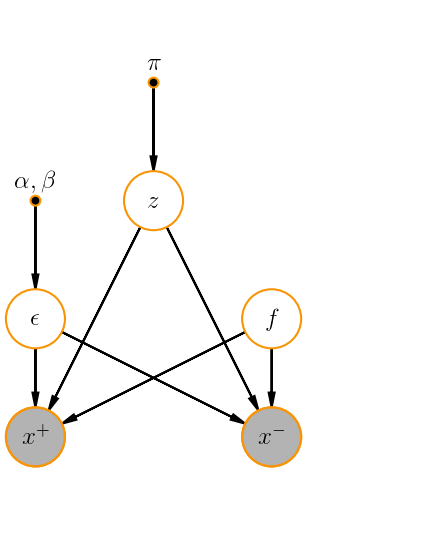
\includegraphics[width=0.3\textwidth]{strand_artifact_pgm.png}
\caption{\label{fig:strand artifact}The probabilistic graphical model for the strand artifact model}
\end{figure}

The strand artifact filter detects sequencing artifacts in which the evidence for the alt allele consists entirely of forward strand reads alone or reverse strand reads alone. We must detect this while taking into account the fact that at some loci, such as near the end of an exome target, \emph{all} reads are biased towards one direction, and therefore a bias towards a particular strand among alt reads is no cause for alarm.

Let $z \in \{ z_+, z_-, z_o \}$ be a latent random variable with 1-hot encoding that represents the artifact state of a suspected variant i.e. $z_+ = 1$ for a forward strand artifact, $z_- = 1$ for a reverse artifact, and $z_o = 1$ otherwise. At each locus, let $x_\pm$ be the number of forward (+) or reverse (-) strand alt reads and let $n_\pm$ be the total depth for each strand.  By modeling $x_\pm$ relative to $n_\pm$ we account for inherent strand bias due to, for example, reads falling at the end of an exome target and do not confuse it for an artifact.  Let $f$ be the allele fraction of true variation in case $z_o = 1$.  Let $\epsilon$ be the strand bias error rate and let $\theta$ be the non-strand-biased error rate.  We will ignore the case in which significant strand bias coincides with real variation, first because this is exceedingly rare and ignoring it has a negligible effect on the parameters of our model, and secondly because such variants should be considered true positives.


The conditional distributions of our model are binomial
\begin{align}
x_+ | \epsilon, \theta, f, z_+ = 1 &\sim \text{Bin} (x_+ | n_+, \epsilon) \\
x_+ | \epsilon, \theta, f, z_- = 1 &\sim \text{Bin} (x_+ | n_+, \theta) \\
x_+ | \epsilon, \theta, f, z_o = 1 &\sim \text{Bin} (x_+ | n_+, f),
\end{align}
and similarly for $x_-$.  Putting beta priors on $\epsilon$, $\theta$, and $f$, with parameters $(\alpha_\epsilon, \beta_\epsilon)$, $(\alpha_\theta, \beta_\theta)$, and $(\alpha_f, \beta_f)$ and marginalizing latent parameters we obtain likelihoods
\begin{align}
P(x_+, x_- | z_\pm = 1) =& \text{BetaBinom}(x_\pm | n_\pm, \alpha_\epsilon, \beta_\epsilon) \text{BetaBinom}(x_\mp | n_\mp, \alpha_\theta, \beta_\theta) \\
P(x_+, x_- | z_o = 1) =& \int_0^1 \text{Beta}(f | \alpha_f, \beta_f) \text{Binom}(x_+ | n_+, f) \text{Binom}(x_- | n_-, f) df \\ 
                                  =& \frac{ \binom{n_+}{x_+} \binom{n_-}{x_-}}{\binom{n_+ + n_-}{x_+ + x_-}} \text{BetaBinom}(x_+ + x_- | n_+ + n_-, \alpha_f, \beta_f)
\end{align}

Finally, we let $\pi/2$ be the prior probability of a forward or reverse strand artifact.  From the above equations it is straightforward to calculate the posterior probability of $z$ and to learn $\pi$ iteratively via the EM algorithm.  It is somewhat more complicated to learn $(\alpha_\epsilon, \beta_\epsilon)$ and $(\alpha_\theta, \beta_\theta)$, so we treat these as fixed hyperparameters.  We use a flat prior $\alpha_f = \beta_f = 1$ for the true allele fraction.

%%%%%%%
%GERMLINE
%%%%%%%
\subsection{Germline Filter}\label{germline-filter}
Suppose we have detected an allele such that its (somatic) likelihood in the tumor is $\ell_t$ and its (diploid) likelihood in the normal is $\ell_n$\footnote{This is the total likelihood for het and hom alt in the normal.}.  By convention, both of these are relative to a likelihood of $1$ for the allele \textit{not} to be found.  If we have no matched normal, $\ell_n = 1$.  Suppose we also have the population allele frequency $f$ of this allele.  Then the prior probabilities for the normal to be heterozygous and homozygous alt for the allele are $2f(1-f)$ and $f^2$ and the prior probability for the normal genotype not to contain the allele is $(1-f)^2$.  Finally, let the prior for this allele to arise as a somatic variant be $\pi$.

If the variant exists in the tumor as a real somatic variant it has likelihood $\ell^S_t$, the adjusted \code{Mutect2} likelihood accounting for allele fraction clustering.  If it exists as a germline het in a segment with minor allele fraction $m$ the likelihood is $\ell_t(m)$ for the alt minor case and $\ell_t(1-m)$ for the alt major case, after adjusted the \code{Mutect2} likelihood toa ccount for pinning the allele fraction to $m$ or $1-m$.  We need the unnormalized probabilities of three possibilities:
\begin{enumerate}
\item The variant exists in the tumor and the normal as a germline het.  This has unnormalized probability $f(1-f) \ell_n (1 - \pi) \left( \ell_t(m) + \ell_t(1 - m) \right)$.
\item The variant exists in the tumor and the normal as a germline hom alt.  This has unnormalized probability $f^2 \ell_n \ell_t(1) (1 - \pi)$.
\item The variant exists in the tumor but not the normal.  This has unnormalized probability $(1-f)^2 \ell^S_t \pi$.
\end{enumerate}

We exclude possibilities in which the variant does not exist in the tumor sample because we really want the conditional probability that the variant is germline given that it would otherwise be called.  The normalized sun of the first two possibilities is the germline error probability.

So far we have assumed that the population allele frequency $f$ is known, which is the case if it is found in our germline resource, such as gnomAD.  If $f$ is not known we must make a reasonable guess as follows.  Suppose the prior distribution on $f$ is ${\rm Beta}(\alpha, \beta)$.  The mean $\alpha/(\alpha +\beta)$ of this prior is the average human heterozygosity $\theta \approx 10^{-3}$, so we have $\beta \approx \alpha / \theta$.  We need one more constraint to determine $\alpha$ and $\beta$, and since we are concerned with imputing $f$ when $f$ is small we use a condition based on rare variants.  Specifically, the number of variant alleles $n$ at some site in a germline resource with $N/2$ samples, hence $N$ chromosomes, is given by $f \sim {\rm Beta}(\alpha, \beta), n \sim {\rm Binom}(N,f)$.  That is, $n \sim {\rm BetaBinom}(\alpha, \beta, N)$.  The probability of a site being non-variant in every sample is then $P(n = 0) = {\rm BetaBinom}(0 | \alpha, \beta, N)$, which we equate to the empirical proportion of non-variant sites in our resource, about $7/8$ for exonic sites in gnomAD.  Solving, we obtain approximately $\alpha = 0.01, \beta = 10$ for gnomAD.  Now, given that some allele found by \code{Mutect2} is not in the resource, the posterior on $f$ is ${\rm Beta}(\alpha, \beta + N)$, the mean of which is, since $\beta << N$, about $\alpha / N$.  By default, \code{Mutect2} uses this value.

%%%%%%%%%%
%CONTAMINATION
%%%%%%%%%%
\subsection{Contamination Filter}\label{contamination-filter}
Suppose our tumor sample has contamination fraction $\alpha$ and that at some site we have $a$ alt reads out of $d$ total reads.  Suppose further that the alt allele has population allele frequency $f$.  We estimate the probability that these alt reads came from a contaminating sample and not from a true somatic variant.  Let $\pi$ be the prior probability of a somatic variation from the allele fraction clustering model.  Then alt read count likelihood $P(a | d, {\rm somatic})$ is also given by this model.  The possibility that the reads are due to contamination has prior $1 - \pi$ and we take the maximum likelihood among two models of contamination.

If there are multiple contaminants we approximate each contaminant read as independent so that
\begin{equation}
P(a | d, {\rm many~contaminant}) = {\rm Binom}(a | d, \alpha f).
\end{equation}
If there is a single contaminating sample it is heterozygous with probability $2f(1-f)$ and homozygous for the alt with probability $f^2$, in which cases fractions $\alpha/2$ and $\alpha$ of all reads to be alt contaminants.  The contaminant is homozygous for the ref with probability $(1-f)^2$, which yields no alt reads. Thus
\begin{equation}
P(a | d, {\rm one~contaminant}) = 2f(1-f) {\rm Binom}(a | d, \alpha /2) + f^2 {\rm Binom}(a | d, \alpha) + (1-f)^2 {\rm I}[a = 0].
\end{equation}
Taking the maximum of these as the likelihood given contamination, we can easily compute the probability of contamination error.

%%%%%%%%%%%%%
%READ ORIENTATION
%%%%%%%%%%%%%
\subsection{Read Orientation Artifact Filter}
The read orientation model is implemented in \code{LearnReadOrientationModel}, which produces the  \code{--orientation-bias-artifact-priors} input to \code{FilterMutectCalls}.  The raw counts for code{LearnReadOrientationModel} are generated either by \code{CollectF1R2Counts} or \code{Mutect2} itself.

\begin{lstlisting}[language=bash,caption={LearnReadOrientationModel command}, label={cmd-mutect2}]
gatk Mutect2 -R reference.fasta \
   -I tumor.bam \
   -O unfiltered.vcf \
   [. . . any other arguments] \
   --f1r2-tar-gz f1r2.tar.gz
   
gatk LearnReadOrientationModel \
   -I f1r2.tar.gz
   -O tumor-artifact-prior.tar.gz
\end{lstlisting}
The output \code{tumor-artifact-prior.tar.gz} is then passed as the parameter to \code{FilterMutectCalls} with the \code{--orientation-bias-artifact-priors} argument.  Note that all tar.gz files shown above contain information for every tumor sample input to \code{Mutect2}.

The read orientation artifact, also known as the orientation bias artifact, arises due to a chemical change in the nucleotide during library prep that results in, for example, G base-paring with A. This kind of artifact has a clear signature (e.g. C to A SNP that occurs predominantly for the middle C in the DNA sequence CCG), and it's single-stranded in nature. Downstream, this artifact manifests as low allele fraction SNPs whose evidence for the alt allele consists almost entirely F1R2 reads or F2R1 reads. A read pair is F1R2 (forward 1st, reverse 2nd) if the sequence of bases in Read 1 maps to the forward strand of the reference (F1), and the sequence of Read 2 to the reverse strand of the reference (R2). F2R1 is defined similarly.

Without loss of generality, suppose that the reference context at locus $i$ is ACT. Let $\vz_i$ denote the genotype at locus $i$ with the one-hot encoding $z_{ik} = 1$ iff the genotype of locus $i$ is $k$, where the possible genotypes are
\begin{equation*}
z_i \in \{ \text{F1R2}_A, \text{F1R2}_G, \text{F1R2}_T, \text{F2R1}_A, \text{F2R1}_G, \text{F2R1}_T,  \text{Hom Ref}, \text{Germline Het}, \text{Somatic Het}, \text{Hom Var} \}
\end{equation*}
$z_i = \mathrm{F1R2_A}$ denotes that at locus $i$ we have an artifact in which the evidence for alt allele A consists entirely of reads in the F1R2 orientation. The remaining artifact states are defined analogously. Let $\vpi$ denote the prior probabilities of the $\vz_i$ under the reference context ACT. Then we have 
\begin{equation}
P(\vz_i) = \prod_k \pi_{k}^{z_{ik}}
\end{equation}

The number of alt reads at a locus depends on the genotype $z_i$. Let $n_i$ and $m_i$ denote the total depth and alt depth at locus $i$, respectively. The conditional distribution of $m_i$ is
\begin{equation}
P(m_i | z_{ik} = 1) = \mathrm{BetaBinomial}(m_i | n_i, \alpha_k, \beta_k)
\end{equation}
where $\alpha_k$ and $\beta_k$ are fixed hyperparameters for genotype $z_k$. When the site's genotype indicates in $m_i$ alt reads we expect a heavily skewed distribution of F1R2 reads. This is captured in the conditional distribution of F1R2 alt reads. Let $c_i$ denote the number of F1R2 reads among the $m_i$ alt reads at locus $i$. Then we have
\begin{equation}
P(c_i | m_i, z_{ik} = 1) = \mathrm{BetaBinomial}( c_i | m_i, \alpha'_k, \beta'_k)
\end{equation}
We learn the prior artifact probabilities $\vpi$ based on the observed values of $n_i$, $m_i$, $c_i$ for each of $N$ loci using the EM algorithm. In the E-step, we compute the posterior probabilities of $\vz_i$ for $i = 1 ... N$. The joint probabilities of $\vz$ factorizes over $i$, thus the posteriors over $\vz$ are independent across loci. 
\begin{equation}
P(z_{ik} = 1 | m_i, c_i) \propto P(z_{ik} = 1, m_i, c_i) = \pi_{k} \mathrm{BetaBinomial}(m_i | n_i, \alpha_k, \beta_k)  \mathrm{BetaBinomial}( c_i | m_i, \alpha'_k, \beta'_k)
\end{equation}
In the M-step we maximize the expectation of the log complete-data likelihood with respect to $\vpi$. The log complete data likelihood is given as
\begin{equation}
\ln P(\vz, \vm, \vc) = \sum_i \sum_k z_{ik} \big( \ln \pi_{k} + \ln \mathrm{BetaBinomial} ( m_i | n_i, \alpha_k, \beta_k)  + \ln \mathrm{BetaBinomial}( c_i | m_i, \alpha'_k, \beta'_k) \big)
\end{equation}
Maximizing the log likelihood under the constraint $\sum_k \pi_k = 1$ gives us
\begin{equation}
\pi_k = \frac{N_k}{N}
\end{equation}
where $N_k = \sum_i P(z_{ik} | m_i, c_i)$ is the effective count of loci with genotype $k$. We alternate E-step and M-step until convergence. We then use the learned prior genotype probabilities to compute the posterior artifact probabilities of variants in a vcf. The filtering threshold is set such that the false discovery rate doesn't exceed a specified value, as described below.

%%%%%%%%%%%%%%
%POLYMERASE SLIPPAGE
%%%%%%%%%%%%%%
\subsection{Polymerase Slippage}\label{polymerase-slippage}
For indels in short tandem repeats (STRs) \code{FilterMutectCalls} uses a simple model for the possibility that alt reads are due to polymerase slippage.  The prior $\pi_L$ for a real variant of length $L$ comes from the allele fraction clustering model.  \code{FilterMutectCalls} assumes that polymerase slippage only occurs in STRs of 8 bases or more and only results in insertions or deletions of a single repeat unit.  The likelihood of $a$ alt reads out of $d$ total reads in the case of a real somatic variant is given by the allele fraction clustering model.  The likelihood in the case of polymerase slippage is the marginal of binomial likelihoods over a slippage rate with a uniform prior from 0 to $0.1$, which is a regularized Beta function.  Given priors and likelihoods, the error probability follows.

%%%%%%%%%%%%%%
%NORMAL ARTIFACT
%%%%%%%%%%%%%%
\subsection{Normal Artifacts}\label{normal-artifact}
A matched normal is useful not only for detecting germline variants but also for distinguishing technical artifacts for somatic mutations.  Even a large panel of normals may not include, for example, mapping errors due to a rare SNP in a centromere, while a matched normal will exhibit such errors.  \code{Mutect2} emits a normal artifact log odds annotation by applying the somatic likelihoods model to the normal.  We combine this likelihood of the reads given that an artifact appears in the normal with a prior probability for normal artifacts to obtain a posterior error probability.  Since this prior is unknown, we use the rate of technical artifacts in the tumor detected by \code{FilterMutectCalls} as a proxy.

%%%%%%%%%%%%%%
%BAD HAPLOTYPE
%%%%%%%%%%%%%%
\subsection{Bad Haplotypes}\label{bad-haplotype}
\code{Mutect2} emits phasing information for calls in the same assembly region.  We assign a ``bad haplotype" probability equal to the greatest technical artifact probability of any in-phas call within a certain distance, by default 100 bases.


%%%%%%%%%%%%%
%%%%%%%%%%%%%
%RELATED GATK TOOLS
%%%%%%%%%%%%%
%%%%%%%%%%%%%
\section{Related GATK Tools}
The Broad somatics SNVs and indels pipeline involves several GATK tools besides \code{Mutect2} and \code{FilterMutectCalls}.  We describe them here.

\subsection{Creating a Panel of Normals}
Currently, a panel of normals is simply a vcf of blacklisted sites flagged as recurrent artifacts\footnote{\code{CreateSomaticPanelOfNormals} emits more information than this, but \code{Mutect2} does not yet use it.}.  One generates it by running \code{Mutect2} in tumor-only mode on a large number of normal samples, then running the following workflow:

\begin{lstlisting}[language=bash,caption={CreateSomaticPanelOfNormals command}, label={cmd-mutect2}]
gatk GenomicsDBImport -R reference.fasta -L intervals.interval_list \
   --genomicsdb-workspace-path pon_db \
   -V normal1.vcf \
   -V normal2.vcf \
   -V normal3.vcf . . .
   
gatk CreateSomaticPanelOfNormals -R reference.fasta -V gendb://pon_db -O pon.vcf
\end{lstlisting}



\subsection{Calculating Contamination}
To calculate the cross-sample calculation of a tumor sample, one runs the GATK tools \code{GetPileupSummaries} and \code{CalculateContamination} as follows:

\begin{lstlisting}[language=bash,caption={CalculateContamination command}, label={cmd-mutect2}]
gatk GetPileupSummaries -I tumor.bam \
   -V common-biallelic.vcf \
   -L common-biallelic.vcf \
   -O tumor.pileups

# if a normal is present, it is helpful to obtain its pileup sumaries
gatk GetPileupSummaries -I normal.bam \
   -V common-biallelic.vcf \
   -L common-biallelic.vcf \
   -O tumor.pileups

gatk CalculateContamination -I tumor.pileups \
   # the normal pileups are useful but optional
   [-matched normal.pileups] \
   -O contamination.table \
   # it is highly recommended to produce segments for FilterMutectCalls
   [-tumor-segmentation segments.table]
\end{lstlisting}

\code{CalculateContamination} is the GATK's fast, simple, and accurate method for calculating the contamination of a sample.  This methods does not require a matched normal, makes no assumptions about the number of contaminating samples, and remains accurate even when the sample has a lot of copy number variation.

The inputs are a bam file and a vcf of common variants -- for example ExAC, gnomAD, or 1000 Genomes -- with their allele frequencies.  The basic idea, which comes from ContEst\footnote{ContEst: estimating cross-contamination of human samples in next-generation sequencing data, \textit{Bioinformatics} \textbf{27}, 2601 (2011)} by Kristian Cibulskis and others in the Broad Institute Cancer Genome Analysis group, is simply to count ref reads at hom alt sites and subtract the number of ref reads expected from sequencing error to obtain the number of ref reads contaminating these hom alt sites.  Finally, we use the allele frequencies to account for the fact that some contaminating reads have the alt allele.  The only subtlety is in distinguishing hom alt sites from loss of heterozygosity events, which we describe below.

Suppose we have a set $\mathbb{H}$ of SNPs at which our sample is homozygous for the alternate allele.  Let $N_{\rm ref}$ be the total number of ref reads at these sites.  We can decompose $N_{\rm ref}$ as follows:
\begin{align}
N_{\rm ref} = N_{\rm ref}^{\rm error} + N_{\rm ref}^{\rm contamination}, \label{decomposition}
\end{align}
where $N_{\rm ref}^{\rm error}$  and $N_{\rm ref}^{\rm contamination}$ are as the number of ref reads due to error and contamination, respectively.  We can obtain $N_{\rm ref}$ by counting reads, and we estimate $N_{\rm ref}^{\rm error}$ as follows.  Suppose, WLOG, that the ref allele is A and the alt is C.  Then, assuming that all substitution errors are equally likely, $N_{\rm ref}^{\rm error}$ is approximately half the number of Gs and Ts.  This is, of course, not a perfect assumption for any one site, but on average over all the sites in $\mathbb{H}$ it is very good.

Next we take the expectation of both sides of Equation \ref{decomposition} to obtain
\begin{align}
\ave{N_{\rm ref} - N_{\rm ref}^{\rm error}} =& \ave{\sum_{s \in \mathbb{H}} {\rm number~of~contaminant~ref~reads~at~}s} \\
=& \sum_{s \in \mathbb{H}} \ave{{\rm number~of~contaminant~ref~reads~at~}s} \\
=& \sum_{s \in \mathbb{H}} \ave{{\rm number~of~contaminant~reads~at~}s \times {\rm ref~fraction~of~contaminant~reads~at~}s} \\
=& \sum_{s \in \mathbb{H}} \ave{{\rm number~of~contaminant~reads~at~}s} \times \ave{{\rm ref~fraction~of~contaminant~reads~at~}s}
\end{align}
where we have used the linearity of the expectation and the independence of the total number of contaminant reads with the fraction of contaminant reads that are ref.  The expectation of the total number of contaminant reads is the depth $d_s$ at site $s$ times the contamination, which we denote by $\chi$.  The expected fraction of contaminant reads that are ref is one minus the alt allele frequency $f_s$.  Crucially, this fact is independent of how many contaminating samples there are.  Thus we have
\begin{align}
\ave{N_{\rm ref} - N_{\rm ref}^{\rm error}} = \chi \sum_{s \in \mathbb{H}} d_s (1 - f_s)
\end{align}
and obtain the estimate
\begin{align}
\hat{\chi} \approx \frac{N_{\rm ref} - N_{\rm ref}^{\rm error}}{\sum_{s \in \mathbb{H}} d_s (1 - f_s)} \label{contamination_estimate}
\end{align}


Let us now roughly estimate the error bars on this result.  The main source of randomness is the stochasticity in the number of contaminating ref reads.  Although the nature of this randomness depends on the number of contaminants, the most variable case, hence an upper bound, is that of a single haploid contaminant, since at each site the only possibilities are the extremes of all contaminant reads being ref or all being alt.  In this case, the contribution to the numerator of Eq. \ref{contamination_estimate} from site $s$ is the random variable $X_sZ_s$, where $X_s \sim {\rm Binom(d_s, \chi)}$ is the number of contaminant reads at $s$ and $Z_s$ is a binary indicator for whether the contaminant reads are ref, with $P(Z_s=1) = 1 - f_s$.  $X$ and $Z$ are independent, so we can work out the variance of $XZ$ as:
\begin{align}
{\rm var}(XZ) =& E[X^2Z^2] - E[XZ]^2 \\
=& (1 - f_s) E[X^2] - (1-f_s)^2 E[X]^2 \\
=& (1 - f_s) \left( {\rm var}(X) + E[X]^2 \right) - (1 - f_s)^2E[X]^2 \\
=& (1 - f_s) d_s \chi(1 - \chi) + f_s(1 - f_s) d_s^2 \chi^2
\end{align}
And therefore the standard error on $\hat{\chi}$ comes out to the square root of the sum of these per-site variances, divided by the denominator of Eq. \ref{contamination_estimate}, that is,
\begin{equation}
{\rm std}(\hat \chi) = \frac{\sqrt{  \sum_s \left[ (1 - f_s) d_s \hat{\chi}(1 - \hat{\chi}) + f_s(1 - f_s) d_s^2 \hat{\chi}^2  \right] }}{\sum_s d_s (1 - f_s) }
\end{equation}

It remains to describe how we determine which sites are hom alt.  The fundamental challenge here is that in cancer samples loss of heterozygosity may cause het sites to look like hom alt sites.  Our strategy is to partition the genome into allelic copy-number segments, then infer the minor allele fraction of those segments.  We segment the genome just as in GATK CNV, using a kernel segmenter with a Gaussian kernel computed on the alt fraction.  A nonlinear kernel is important because each segment is multimodal, with peaks for hom ref, alt minor het, alt major het, and hom alt.  

We then perform maximum likelihood estimation MLE on a model with learned parameters $\mu$, the local minor allele fraction for each segment, $\chi$, the contamination, and a constant base error rate parameter $\epsilon$ determined by counting reads that are neither the ref nor primary alt base at biallelic SNPs as described above.  The model likelihood is
\begin{equation}
P(\{ a\}| \{f\}, \chi, \{d\}) =    \prod_{{\rm segments~}n}\prod_{{\rm sites~}s} \sum_{{\rm genotype~}g} P(g|f_s) {\rm Binom}(a_s | d_s, (1 - \chi) \phi(g, \mu_n, \epsilon) + \chi f_s)
\end{equation}
where $a_s$ and $d_s$ are the alt and total read counts at site $s$, allelic CNV genotypes $g$ run over hom ref, alt minor, alt major, and hom alt with priors $P({\rm hom~ref}) = (1-f_s)^2$, $P({\rm alt~minor}) = P({\rm alt~major}) = f_s(1-f_s)$, and $P({\rm hom alt} = f^2$.  $\phi(g, \mu, \epsilon)$ is the alt allele fraction of the uncontaminated sample: $\phi({\rm hom~ref}) = \epsilon$, $\phi({\rm alt~minor}) = \mu$, $\phi({\rm alt~major}) = 1 - \mu$, $\phi({\rm hom~alt}) = 1 - \epsilon$.  The binomial is the weighted average of the uncontaminated sample and sample reads drawn independently from allele frequency $f$.  This is inconsistent with a single diploid contaminant sample, or indeed with any finite number of contaminants, which is why we do not the the MLE estimate in the final output of the tool.  The model also assumes that the uncontaminated and contaminating samples have the same overall depth distribution at each site, which is inconsistent with any differences in copy-number.  We perform the MLE by brute force, alternately maximizing with respect to $\chi$ with $\mu$ fixed and vice versa.  In order to make the solution more robust, we exclude segments with low $\mu$ from the maximization over $\chi$ by taking the highest possible threshold (up to 0.5, of course) for $\mu$ that retains at least $1/4$ of all sites.

Once we have learned the parameters of this model, we can easily infer the posterior probabilities of hom alt genotypes.  We take every site with a posterior probability greater than 0.5.  In order to make the result more reliable against CNVs, we again impose a threshold on segment minor allele fraction and apply the above formula only to hom alt sites in these segments.  This time, however, we choose the highest possible threshold such that the estimated relative error is less than 0.2.

Finally, we note that the same calculation can be reversed by using alt reads in hom ref sites as the signal and replacing $f$ by $1-f$ everywhere above.  We use the estimate from hom refs as a backup when the hom alt estimate has too great an error, as can occur in the case of targeted panels with few sites.  We do not use this as our primary estimate because it is much more affected by uncertainty in the population allele frequencies and is thus susceptible to systematic bias.

\subsection{Filtering Alignment Artifacts}
\code{FilterMutectCalls} does a fairly good job detecting all sorts of errors, including mapping artifacts.  When more precision is needed and a slight loss of sensitivity is acceptable, one can run the output of \code{FilterMutectCalls} through \code{FilterAlignmentArtifacts}.  This tool looks at every alt-supporting read together with its mate and maps both to the best reference available\footnote{That is, if the reads come from an hg19-aligned bam, they will still be realigned to hg38 if that is provided.} using an embedded BWA-mem with parameters optimized for detecting multimapping.  The tool requires a BWA mem reference image index file, which is available from the GATK resource bucket.  The first step below, in which this image is generated, is usually not necessary.

\begin{lstlisting}[language=bash,caption={FilterAlignmentArtifacts command}, label={cmd-filter-alignment-artifacts}]
gatk BwaMemIndexImageCreator -I reference.fasta -O reference.fasta.img

gatk FilterAlignmentArtifacts \
   # the reference argument is the bam's original alignment
   -R original-reference.fasta \
   # filtered calls from FilterMutectCalls
   -V filtered.vcf \
   -I tumor.bam \
   --bwa-mem-index-image reference.fasta.img \
   -O realignment-filtered.vcf
\end{lstlisting}


\subsection{Proposed tumor in normal estimation tool}

Note: the following notes are just a proposal for which no GATK tool yet exists.  A popular tool is DeTiN\footnote{DeTiN: overcoming tumor-in-normal contamination, \textit{Nature Methods} \textbf{15}, 531 (2018)} by Amaro Taylor-Weiner and others at the Broad Institute Cancer Genome Analysis group.

Similar to the spirit of CalculateContamination, the fraction of tumor reads in the normal bam is a single number with a large amount of evidence and is probably well-estimated by simple descriptive statistics rather than a full-fledged probabilistic model.  It shouldn't be much more complicated than finding somatic variants and comparing their signal in the normal sample to that in the tumor.

We propose the following steps to obtain our input of confident somatic SNVs:
\begin{itemize}
\item Run \code{Mutect2} with the \code{--genotype-germline-sites} argument to obtain a preliminary list of somatic SNVs, including those that look like germline variants due to tumor-in-normal contamination.  For the sake of speed, we could implement a pileup-based mode in which we skip reassembly and equate read likelihoods with base qualities.  This would allow us to obtain variant annotations using the existing architecture of \code{Mutect2} and therefore to filter calls with no new code.  
\item Run \code{FilterMutectCalls}.  With default settings this eliminates the great majority of sequencing artifacts.  To eliminate even more we could increase the log odds threshold slightly, essentially requiring a slightly larger alt allele count.  Normally we don't do this because it sacrifices some sensitivity, but for our purposes here a 10 or 20 percent loss of sensitivity is perfectly acceptable as long as we are left with enough SNVs for our estimate.  It would also make sense to be especially stringent with variants that have any significant population allele frequency in gnomAD, as well as possible mapping errors.  Thus we might also run FilterAlignmentArtifacts with strict parameters.
\item Reconsider all variants that are filtered only by the germline and/or normal artifact filters.  Those that have enough read counts in the normal that we conclude they are germline variants, as opposed to tumor in normal contamination, should remain filtered.  
\end{itemize}

The above steps are all very reliable, so at this point we can assume we have a collection of confident biallelic somatic SNVs that are hom ref in the germline.  Similar to CalculateContamination, we can now estimate the number of alt reads in the normal at these sites:
\begin{align}
{\rm alt~in~normal} \approx \sum_{\rm sites} ({\rm depth~in~normal}) \times ({\rm alt~fraction~in~tumor}) \times ({\rm tumor~in~normal~fraction})
\end{align}
Hence we estimate
\begin{align}
{\rm tumor~in~normal~fraction} \approx 
\frac{\rm total~number~of~alt~reads~in~normal~at~somatic~SNV~sites}
{\sum_{\rm somatic~SNV~sites} ({\rm depth~in~normal}) \times ({\rm alt~fraction~in~tumor})}
\end{align}

We could also iterate this process as in CalculateContamination: first get an initial guess of the tumor-in-normal fraction, then use the initial guess to improve our ``un-filtering" in the third step above.

\end{document}